%\documentclass[]{beamer}
\documentclass[aspectratio=169]{beamer}
\pdfpkresolution=8000
\usepackage[utf8]{inputenc} % use UTF-8
\usepackage[T2A,OT1]{fontenc} % rus fonts
\usepackage[russian]{babel}

\usepackage{xspace}
\usepackage{lipsum}
\usepackage{standalone}
%\usepackage{ragged2e}
%\justifying

\newcommand{\kmeans}{\mbox{$ k $-means}\xspace}
\newcommand{\Ward}{Ward\xspace}
\newcommand{\AWard}{\mbox{A-Ward}\xspace}
\newcommand{\Wardp}{\mbox{Ward$ _p $}\xspace}
\newcommand{\AWardpb}{\mbox{A-Ward$ _{p\beta} $}\xspace}
\newcommand{\BisectingKmeans}{Bisecting \mbox{k-means}\xspace}
\newcommand{\BiKMR}{\mbox{BiKM-R}\xspace}
\newcommand{\dePDDP}{dePDDP\xspace}
\newcommand{\ikmeans}{\mbox{$ ik $-means}\xspace}
\newcommand{\imwkmeanspb}{\mbox{$ imwk $-means$ _{p\beta} $}\xspace}
\newcommand{\PDDP}{PDDP\xspace}


%\renewcommand{\raggedright}{\leftskip=0pt \rightskip=0pt plus 0cm}
\hyphenpenalty=100000 %%% to turn the hyphenation off

\usetheme[progressbar=frametitle]{metropolis}


%%%%%%%%%%%%%%%%%%%%%%%%%%%%%%%%%%%%%%%%%%%%%%%%%%%%%%%%%%%%%%%%%%%%%%%%%%%
 
 \usepackage{tkz-euclide}
 \usetikzlibrary{shapes,backgrounds}
 
 \newcommand\Star[3][]{%
 	\path[#1] (0  :#3) -- ( 36:#2) 
 	-- (72 :#3) -- (108:#2)
 	-- (144:#3) -- (180:#2)
 	-- (216:#3) -- (252:#2)
 	-- (288:#3) -- (324:#2)--cycle;
 }
 \newcommand\Center[3][]{
 	\begin{scope}[shift = {(#2,#3)}, scale=0.08]
 		\Star[#1]{2}{4}
 	\end{scope}
 }
 
 \newcommand\point[3][]{
 	\begin{scope}[shift = {(#2,#3)}, scale=0.08]
 		\draw[#1] (0,0) circle (1.5);
 	\end{scope}
 }
%%%%%%%%%%%%%%%%%%%%%%%%%%%%%%%%%%%%%%%%%%%%%%%%%%%%%%%%%%%%%%%%%%%%%%%%%%%

\title{Разработка программного обеспечения, ориентированного на пользователя, для проведения кластер-анализа по критерию наименьших квадратов}

\author[Еремейкин П.А. \& Миркин Б.Г.]{
	\texorpdfstring{
	\begin{columns}
		\column{.45\linewidth}
		\raggedleft
		\begin{flushleft}
			Выполнил:\\
			Еремейкин Пётр Александрович\\
			студент группы мНоД16-ТМСС\\
			\href{mailto:eremeykin@gmail.com}{\texttt{eremeykin@gmail.com}}
		\end{flushleft}
		\column{.45\linewidth}
		\begin{flushright}
			Руководитель:\\
			Миркин Борис Григорьевич\\
			д.т.н., профессор\\
			\vspace*{1\baselineskip} 
		\end{flushright}
	\end{columns}
	}
	{Еремейкин \& Миркин}
}
\institute{\vspace{1cm} НИУ ВШЭ\\Июнь 2018}
\date{}



\begin{document}
	\begin{frame}
		\titlepage
	\end{frame}
	
%	\section{Test1}
	\begin{frame}{Постановка задачи кластеризации}
		\parbox{\linewidth}{
				Пусть имеется $ N $ объектов и у каждого объекта определены значения $ V $ признаков. Множество всех объектов $ Y $ можно представить в виде таблицы:
			}
		\begin{equation*}
			Y= \begin{pmatrix} 
			y_{1} \\
			\cdots \\ 
			y_{N} 
			\end{pmatrix}
			= \begin{pmatrix} 
			y_{11} & \cdots  & y_{1V} \\ 
			\cdots & \cdots  & \cdots \\ 
			y_{N1} & \cdots  & y_{NV} 
			\end{pmatrix}
		\end{equation*}
		\parbox{\linewidth}{
			Требуется получить разбиение $ S = \{C_1,\ldots,C_K\} $, состоящее из $ K $ кластеров, которые не пересекаются и 	покрывают всё множество объектов $ Y $. Чёткой формулировки относительно того, что должно быть включено в кластеры не существует.  Общая идея состоит в том чтобы сходные объекты были включены в один кластер, а несходные не принадлежали одному кластеру.
		}

		
	\end{frame}
	
	%%%%%%%%%%%%%%%%%%%%%%%%%%%%
	\begin{frame}{Традиционное решение (\kmeans)}
%		\begin{block}{}
%			\parbox{\linewidth}{
%				
%			}
%		\end{block}

       \begin{columns}
       	
       	\column{0.58\linewidth}

   		\parbox{\linewidth}{
	       	Самый популярный алгоритм кластеризации --- \kmeans. Этот метод основан на поочерёдной минимизации квадратичного критерия по двум группам переменных: центрам кластеров и принадлежности объектов кластерам.
		}

		\vspace*{1\baselineskip} 
       	Недостатки метода:
       	\begin{itemize}
       		\item требует задания числа кластеров
       		\item сильно зависит от инициализации
       		\item плохо работает для зашумлённых данных
	    \end{itemize}
       	
       	\column{0.38\linewidth}
       	\centering
       	\vspace{-.4cm}
       	\begin{figure}
       	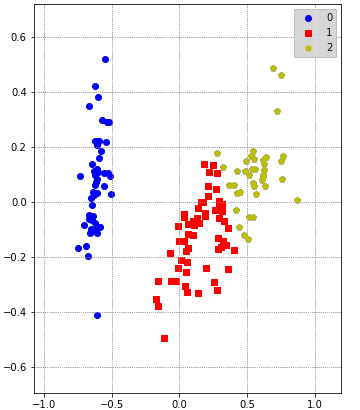
\includegraphics[scale=0.45]{img/iris-kmeans-svd}

		\end{figure}
       \end{columns} 

	\end{frame}

	\begin{frame}{Предлагаемый состав программы}

		\parbox{\linewidth}{За последнее время появилось большое число новых и эффективных алгоритмов кластеризации, многие из них еще не реализованы в популярных библиотеках, таких как \texttt{scipy} для языка Python или  \texttt{Clustering Toolbox} для MATLAB. Предлагается разработать программу, в которую входили бы следующие алгоритмы:}
		
       	\begin{itemize}
       		\item \ikmeans
       		\item \AWard
       		\item \AWardpb
       		\item \dePDDP
	       	\item \BiKMR
       	\end{itemize}
	
	\end{frame}

	
	\begin{frame}{\ikmeans 1}
			\begin{figure} % \ContinuedFloat
				\centering
				\includestandalone[height=0.9\textheight]{img/tikz/ik-means/ik-means-1}
			\end{figure}
	\end{frame}
	
	\begin{frame}{\ikmeans 2}
		\begin{figure} % \ContinuedFloat
			\centering
			\includestandalone[height=0.9\textheight]{img/tikz/ik-means/ik-means-2}
		\end{figure}
	\end{frame}
	
	\begin{frame}{\ikmeans 3}
		\begin{figure} % \ContinuedFloat
			\centering
			\includestandalone[height=0.9\textheight]{img/tikz/ik-means/ik-means-3}
		\end{figure}
	\end{frame}
		
	\begin{frame}{\ikmeans 4}
		\begin{figure} % \ContinuedFloat
			\centering
			\includestandalone[height=0.9\textheight]{img/tikz/ik-means/ik-means-4}
		\end{figure}
	\end{frame}	
	
		
	\begin{frame}{\ikmeans 5}
		\begin{figure} % \ContinuedFloat
			\centering
			\includestandalone[height=0.9\textheight]{img/tikz/ik-means/ik-means-5}
		\end{figure}
	\end{frame}		
		
	\begin{frame}{\ikmeans 6}
		\begin{figure} % \ContinuedFloat
			\centering
			\includestandalone[height=0.9\textheight]{img/tikz/ik-means/ik-means-6}
		\end{figure}
	\end{frame}		
		
	\begin{frame}{\ikmeans 7}
		\begin{figure} % \ContinuedFloat
			\centering
			\includestandalone[height=0.9\textheight]{img/tikz/ik-means/ik-means-7}
		\end{figure}
	\end{frame}		
	
	\begin{frame}{\ikmeans 8}
		\begin{figure} % \ContinuedFloat
			\centering
			\includestandalone[height=0.9\textheight]{img/tikz/ik-means/ik-means-8}
		\end{figure}
	\end{frame}		
	
	\begin{frame}{\ikmeans 9}
		\begin{figure} % \ContinuedFloat
			\centering
			\includestandalone[height=0.9\textheight]{img/tikz/ik-means/ik-means-9}
		\end{figure}
	\end{frame}	
			
	\begin{frame}{\ikmeans 10}
		\begin{figure} % \ContinuedFloat
			\centering
			\includestandalone[height=0.9\textheight]{img/tikz/ik-means/ik-means-10}
		\end{figure}
	\end{frame}			
	
	\begin{frame}{\ikmeans 11}
		\begin{figure} % \ContinuedFloat
			\centering
			\includestandalone[height=0.9\textheight]{img/tikz/ik-means/ik-means-11}
		\end{figure}
	\end{frame}			
	
	\begin{frame}{\ikmeans 12}
		\begin{figure} % \ContinuedFloat
			\centering
			\includestandalone[height=0.9\textheight]{img/tikz/ik-means/ik-means-12}
		\end{figure}
	\end{frame}
	
	\begin{frame}{\ikmeans 13}
		\begin{figure} % \ContinuedFloat
			\centering
			\includestandalone[height=0.9\textheight]{img/tikz/ik-means/ik-means-13}
		\end{figure}
	\end{frame}	
	
	\begin{frame}{\ikmeans 14}
		\begin{figure} % \ContinuedFloat
			\centering
			\includestandalone[height=0.9\textheight]{img/tikz/ik-means/ik-means-14}
		\end{figure}
	\end{frame}	

	\begin{frame}{\ikmeans 15}
		\begin{figure} % \ContinuedFloat
			\centering
			\includestandalone[height=0.9\textheight]{img/tikz/ik-means/ik-means-15}
		\end{figure}
	\end{frame}	
	
	\begin{frame}{\ikmeans 16}
		\begin{figure} % \ContinuedFloat
			\centering
			\includestandalone[height=0.9\textheight]{img/tikz/ik-means/ik-means-16}
		\end{figure}
	\end{frame}	
	
	\begin{frame}{\ikmeans 17}
		\begin{figure} % \ContinuedFloat
			\centering
			\includestandalone[height=0.9\textheight]{img/tikz/ik-means/ik-means-17}
		\end{figure}
	\end{frame}	
	
	\begin{frame}{\ikmeans 18}
		\begin{figure} % \ContinuedFloat
			\centering
			\includestandalone[height=0.9\textheight]{img/tikz/ik-means/ik-means-18}
		\end{figure}
	\end{frame}	

	\begin{frame}{\ikmeans 19}
		\begin{figure} % \ContinuedFloat
			\centering
			\includestandalone[height=0.9\textheight]{img/tikz/ik-means/ik-means-19}
		\end{figure}
	\end{frame}	

	\begin{frame}{\ikmeans 20}
		\begin{figure} % \ContinuedFloat
			\centering
			\includestandalone[height=0.9\textheight]{img/tikz/ik-means/ik-means-20}
		\end{figure}
	\end{frame}	
	
	\begin{frame}{\ikmeans 21}
		\begin{figure} % \ContinuedFloat
			\centering
			\includestandalone[height=0.9\textheight]{img/tikz/ik-means/ik-means-21}
		\end{figure}
	\end{frame}	
		
	\begin{frame}{\ikmeans 22}
		\begin{figure} % \ContinuedFloat
			\centering
			\includestandalone[height=0.9\textheight]{img/tikz/ik-means/ik-means-22}
		\end{figure}
	\end{frame}	
	
		
	\begin{frame}{\ikmeans 23}
		\begin{figure} % \ContinuedFloat
			\centering
			\includestandalone[height=0.9\textheight]{img/tikz/ik-means/ik-means-23}
		\end{figure}
	\end{frame}	

	
%	\begin{frame}{\ikmeans 15}
%		\begin{figure} % \ContinuedFloat
%			\centering
%			\includestandalone[height=0.9\textheight]{img/tikz/ik-means/ik-means-15}
%		\end{figure}
%	\end{frame}	
%	
%	
%	\begin{frame}{\ikmeans 16}
%		\begin{figure} % \ContinuedFloat
%			\centering
%			\includestandalone[height=0.9\textheight]{img/tikz/ik-means/ik-means-16}
%		\end{figure}
%	\end{frame}	
%	
%	\begin{frame}{\ikmeans 17}
%		\begin{figure} % \ContinuedFloat
%			\centering
%			\includestandalone[height=0.9\textheight]{img/tikz/ik-means/ik-means-17}
%		\end{figure}
%	\end{frame}		
%	
%	\begin{frame}{\ikmeans 18}
%		\begin{figure} % \ContinuedFloat
%			\centering
%			\includestandalone[height=0.9\textheight]{img/tikz/ik-means/ik-means-18}
%		\end{figure}
%	\end{frame}		
%	
%	\begin{frame}{\ikmeans 19}
%		\begin{figure} % \ContinuedFloat
%			\centering
%			\includestandalone[height=0.9\textheight]{img/tikz/ik-means/ik-means-19}
%		\end{figure}
%	\end{frame}		
%			
%	\begin{frame}{\ikmeans 20}
%		\begin{figure} % \ContinuedFloat
%			\centering
%			\includestandalone[height=0.9\textheight]{img/tikz/ik-means/ik-means-20}
%		\end{figure}
%	\end{frame}	
%		
%	\begin{frame}{\ikmeans 21}
%		\begin{figure} % \ContinuedFloat
%			\centering
%			\includestandalone[height=0.9\textheight]{img/tikz/ik-means/ik-means-21}
%		\end{figure}
%	\end{frame}	
%	
%	
%	
%	\begin{frame}{\ikmeans 22}
%		\begin{figure} % \ContinuedFloat
%			\centering
%			\includestandalone[height=0.9\textheight]{img/tikz/ik-means/ik-means-22}
%		\end{figure}
%	\end{frame}	
	
	
	
	
		
	\begin{frame}{Система с точки зрения пользователя}
		
	\end{frame}
	
	\begin{frame}{Внутренняя организация}
		
	\end{frame}
	
	\plain{	
		\textsc{Выводы}
		\begin{enumerate}
			\item Создана работоспособная программа
			\item Созданную программу надо опробовать в реальных условиях
		\end{enumerate}
		}	
	\plain{
		\textsc{Спасибо за внимание}!
		}
	

	
\end{document}


